\documentclass{article}

% if you need to pass options to natbib, use, e.g.:
%     \PassOptionsToPackage{numbers, compress}{natbib}
% before loading neurips_2026

% We use the preprint option to compile with proper headers/footers for arXiv or course submission
\usepackage[preprint]{neurips_2026}

\usepackage[utf8]{inputenc} % allow utf-8 input
\usepackage[T1]{fontenc}    % use 8-bit T1 fonts
\usepackage{hyperref}       % hyperlinks
\usepackage{url}            % simple URL typesetting
\usepackage{booktabs}       % professional-quality tables
\usepackage{amsfonts}       % blackboard math symbols
\usepackage{nicefrac}       % compact symbols for 1/2, etc.
\usepackage{microtype}      % microtypography
\usepackage{xcolor}         % colors
\usepackage{graphicx}       % embedding figures
\usepackage{amsmath}        % mathematical equations

\title{Machine Learning for Minute 1 COVID-19 Clinical Triage: A Preattentive Visual Analytics and Fairness Assessment}

\author{%
  Diego Garcés \\
  Applied Machine Learning Division\\
  \texttt{diego.garces@university.edu} \\
}

\begin{document}

\maketitle

\begin{abstract}
During high-volume epidemiological surges, emergency triage personnel must rapidly determine whether arriving patients require immediate hospital admission or can be safely discharged for outpatient care. When evaluating potentially life-threatening respiratory illnesses such as COVID-19 during \emph{Minute 1} of intake, models that inadvertently incorporate post-admission outcomes (e.g., intubation or ICU transfer) suffer from severe data leakage, inflating theoretical accuracy while failing in real-world clinical deployment. In this study, we develop and evaluate an end-to-end Machine Learning decision support pipeline trained on $263,007$ stratified patient arrivals from the official Mexican Epidemiological Surveillance System (SISVER). We enforce a rigorous methodological audit to eliminate post-triage variables and address a $3.2:1$ class imbalance ($23.6\%$ hospitalization rate) by optimizing directly for Precision-Recall Area Under the Curve ($\text{PR-AUC}$). Our tuned Random Forest classifier achieves a $\text{PR-AUC}$ of $0.5771$ ($+132\%$ over the dummy baseline) and captures $70.1\%$ of severe hospitalized arrivals ($\text{Recall}$) on a locked test vault of $52,602$ patients. Coupling state-of-the-art Visual Analytics (InfoVis) with honest subgroup error analysis reveals critical demographic vulnerabilities: young adults ($20\text{--}39$ years old) and patients with zero recorded comorbidities exhibit high false-negative rates ($82.0\%$ and $53.9\%$, respectively). We propose an operational triage protocol combining model-driven probability scores with mandatory pulse oximetry monitoring for young arrivals.
\end{abstract}

\section{Introduction and Clinical Motivation}
\label{sec:introduction}

When a patient arrives at an emergency department or primary care triage station with suspected COVID-19 symptoms, clinical practitioners face a high-stakes decision under tight time constraints: \emph{Should the patient be admitted to an inpatient hospital bed, or can they safely recover at home as an outpatient?} Making an incorrect decision carries asymmetric risks. Sending a severe patient home without medical observation (a False Negative) can lead to rapid respiratory failure and fatality, whereas admitting a mild outpatient for clinical observation (a False Positive) incurs an operational and economic cost but preserves patient safety.

Machine Learning (ML) algorithms offer substantial utility in augmenting clinical decision-making during high-volume surges. However, three fundamental challenges complicate real-world adoption:
\begin{enumerate}
    \item \textbf{Data Leakage:} Many retrospective medical studies inadvertently incorporate variables that are only measured hours or days after admission (e.g., mechanical ventilation or ICU transfer), yielding artificially perfect predictive scores that collapse upon prospective triage deployment.
    \item \textbf{Class Imbalance and Metric Misalignment:} In typical emergency cohorts, mild outpatients outnumber severe hospitalizations. Models evaluated via standard Accuracy tend to predict the majority outpatient class overwhelmingly, missing critical emergencies.
    \item \textbf{Opaque Failure Modes:} Complex tree ensembles or neural networks can mask severe systematic biases across demographic subgroups (e.g., age cohorts or geographic regions) unless evaluated through transparent visual analytics.
\end{enumerate}

To overcome these barriers, we construct a publication-grade, interpretable ML workflow that operates strictly on \emph{Minute 1} intake data. By combining preattentive Visual Analytics (InfoVis) with stratified cross-validation and subgroup error auditing, we provide a robust decision-support framework tailored for high-stakes emergency triage.

\section{Dataset Structure and Methodological Anti-Leakage Audit}
\label{sec:data}

We analyze the official open surveillance dataset provided by the Ministry of Health of Mexico under the Epidemiological Surveillance System for Viral Respiratory Diseases (SISVER) (\texttt{mexico\_covid19.csv}). The raw registry contains $3,846,654$ historical patient records spanning $41$ clinical, demographic, and administrative columns. We filter the cohort to confirmed positive COVID-19 cases and extract a reproducible, stratified random sample of $n=263,007$ patients to conduct rigorous experimentation while preserving statistical fidelity.

\subsection{Target Formulation}
The prediction objective is formulated as a binary classification problem based on the original \texttt{TIPO\_PACIENTE} field:
\begin{itemize}
    \item $\textbf{0}$ (\textbf{Outpatient / Mild}): Patient exhibited moderate symptoms and was sent home for ambulatory recovery ($76.4\%$ of cohort).
    \item $\textbf{1}$ (\textbf{Hospitalized / Severe}): Patient required immediate hospital admission due to high clinical risk ($23.6\%$ of cohort).
\end{itemize}

\subsection{Strict Anti-Leakage Audit}
To ensure strict clinical realism at Minute 1 of intake, we conduct a systematic audit of all available columns, categorizing features into pre-admission predictors versus post-admission outcomes. The following features were explicitly excluded to prevent data leakage:
\begin{itemize}
    \item \textbf{UCI} (Intensive Care Unit admission): Determined days after triage once the patient's inpatient trajectory deteriorates.
    \item \textbf{INTUBADO} (Mechanical intubation): An invasive inpatient procedure ordered after admission is established.
    \item \textbf{FECHA\_DEF} (Date of death): A future survival outcome entirely unknown at initial intake.
    \item \textbf{RESULTADO} (RT-PCR laboratory confirmation): Molecular testing results typically require $24\text{--}72$ hours to process and cannot inform immediate intake triage.
    \item \textbf{NEUMONIA} (Pneumonia diagnosis): Within the SISVER registry, pneumonia confirmation requires chest X-ray or CT imaging performed inside the hospital facility post-admission. Although pneumonia can exist upon arrival, coding conventions make it indistinguishable from hospital-diagnosed complications.
\end{itemize}

Our final validated input feature set comprises exactly $13$ variables: patient age (\texttt{EDAD}), biological sex (\texttt{SEXO}), intake healthcare entity (\texttt{ENTIDAD\_UM}), and $10$ pre-existing chronic comorbidities (\texttt{DIABETES}, \texttt{HIPERTENSION}, \texttt{OBESIDAD}, \texttt{EPOC}, \texttt{ASMA}, \texttt{RENAL\_CRONICA}, \texttt{CARDIOVASCULAR}, \texttt{INMUSUPR}, \texttt{TABAQUISMO}, and \texttt{OTRA\_COM}).

\section{Visual Analytics and Preprocessing Architecture}
\label{sec:infovis}

Rather than applying ad-hoc transformations, our preprocessing pipeline is guided directly by preattentive Visual Analytics (Figure~\ref{fig:data_quality}).

\begin{figure}[htbp]
  \centering
  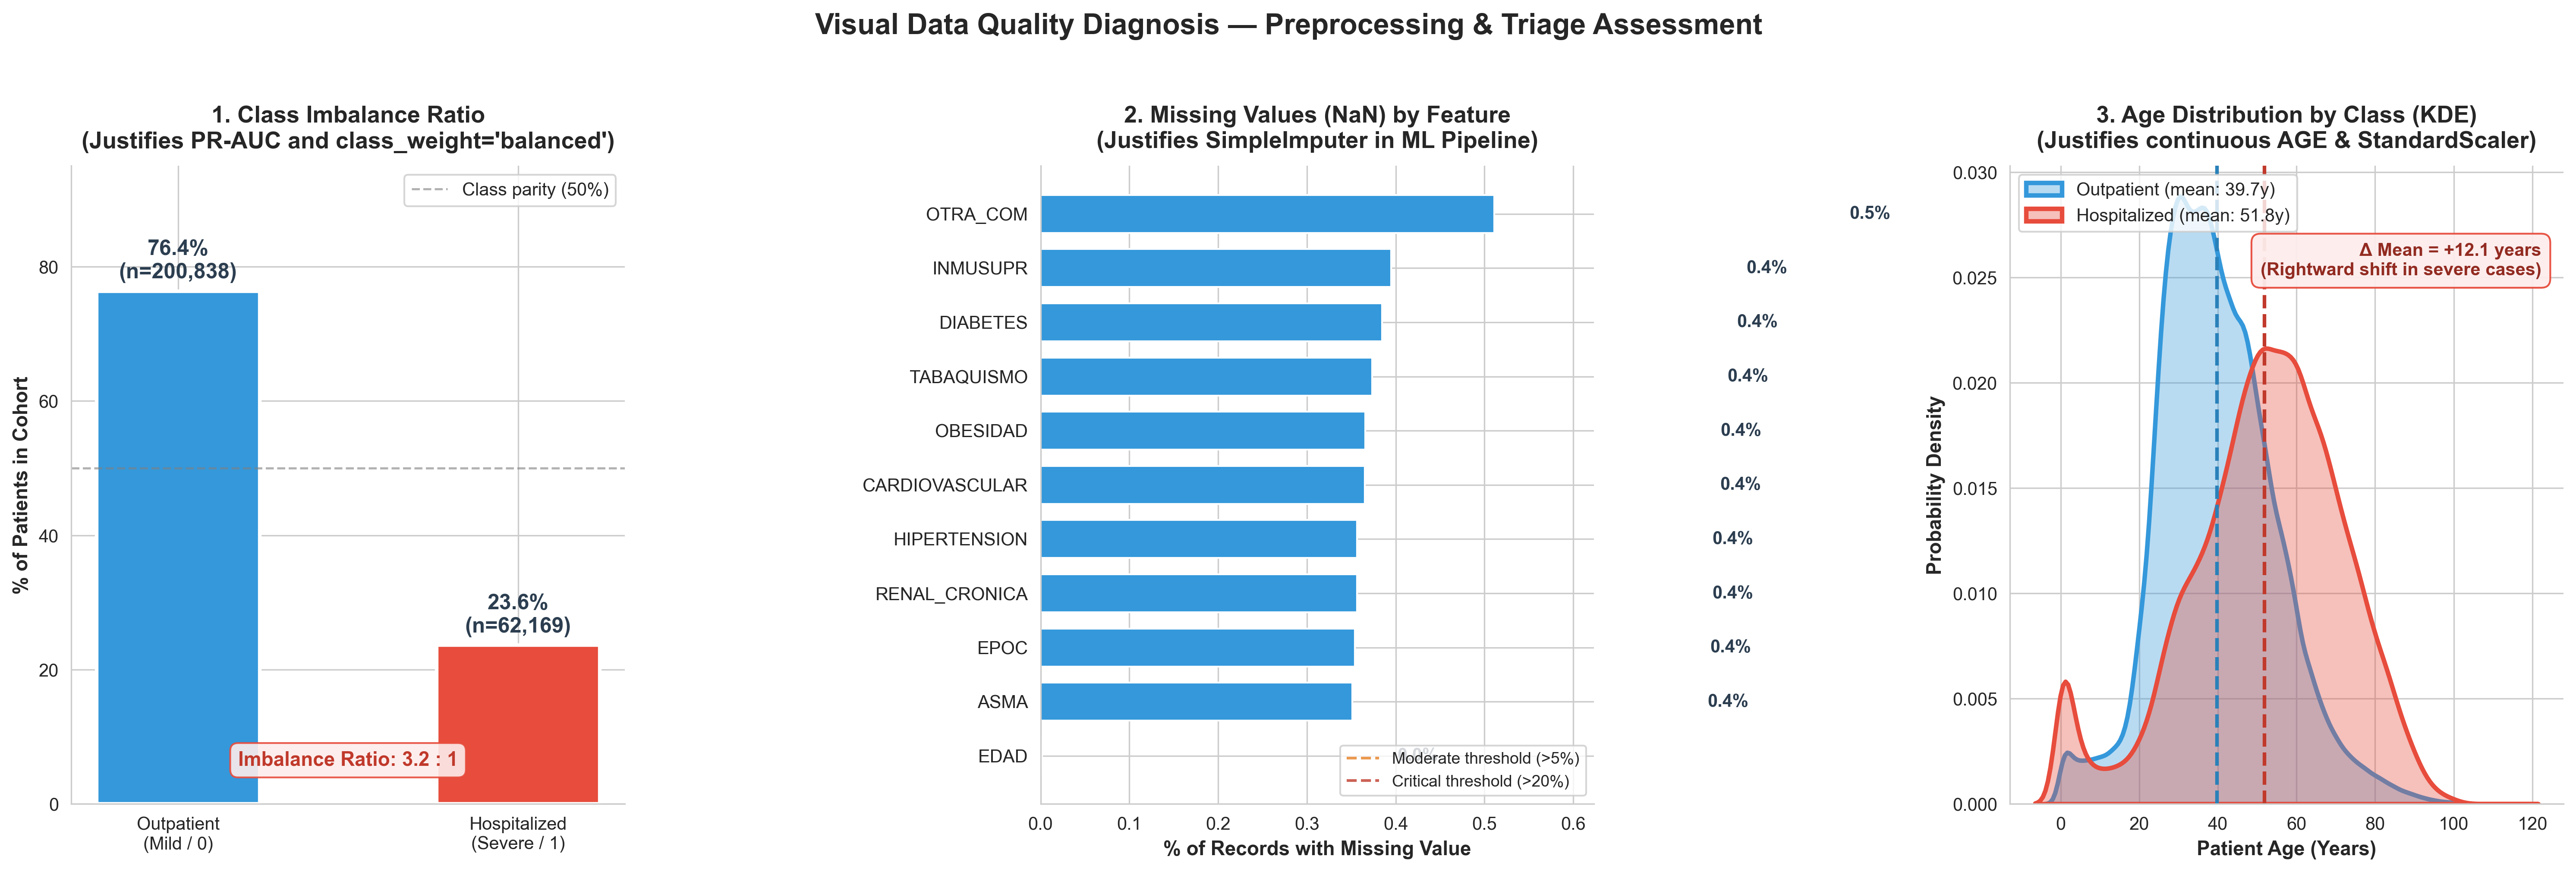
\includegraphics[width=\textwidth]{data_quality_diagnosis.png}
  \caption{\textbf{Visual Data Quality Diagnosis.} Panel 1 demonstrates the $3.2:1$ class imbalance ($23.6\%$ severe), justifying $\text{PR-AUC}$ as our primary evaluation metric and class weighting in tree ensembles. Panel 2 highlights feature missingness profiles, motivating median imputation for age and constant zero imputation for unrecorded comorbidities. Panel 3 shows a $+12.1$-year rightward age shift across hospitalized patients via kernel density estimation, motivating continuous scaling via \texttt{StandardScaler}.}
  \label{fig:data_quality}
\end{figure}

\subsection{Exploratory Risk Factor Analysis}
Visualizing empirical hospitalization rates across demographic and clinical dimensions reveals non-linear risk escalations (Figure~\ref{fig:eda}). Age demonstrates a sharp exponential surge: hospitalization rates remain below $15\%$ for cohorts younger than $40$ years but escalate rapidly past age $50$, exceeding $60\%$ among patients over $70$ years old. Furthermore, specific pre-existing comorbidities act as potent individual multipliers: patients with chronic renal disease (\texttt{RENAL\_CRONICA}) experience a $66.8\%$ admission rate ($+182\%$ relative excess versus the overall cohort mean), while Chronic Obstructive Pulmonary Disease (\texttt{EPOC}) and immunosuppression (\texttt{INMUSUPR}) yield $62.7\%$ and $54.9\%$ admission rates, respectively.

\begin{figure}[htbp]
  \centering
  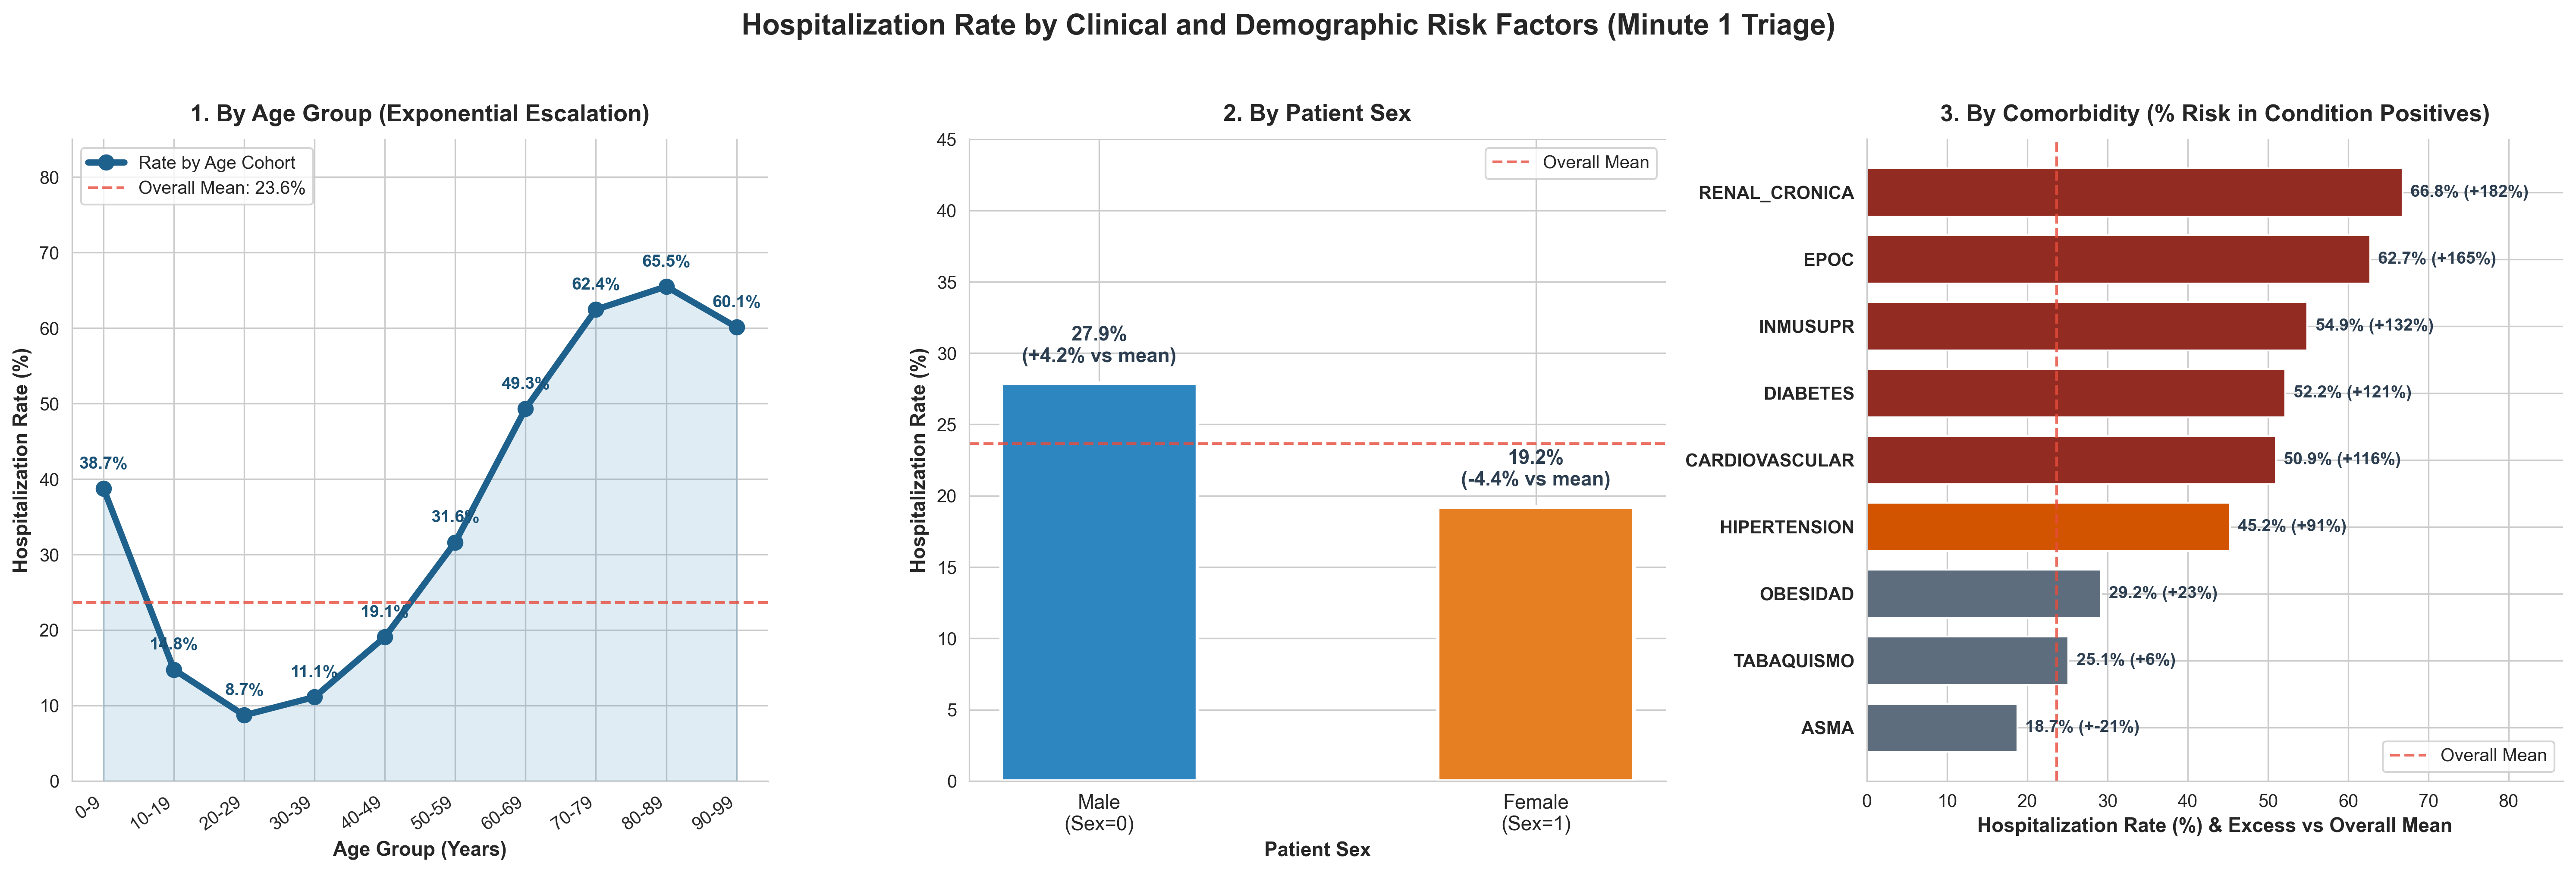
\includegraphics[width=\textwidth]{eda_factores_riesgo.png}
  \caption{\textbf{Minute 1 Clinical Risk Factors.} Panel 1 illustrates the exponential escalation of hospitalization rates by age cohort. Panel 2 highlights sex disparities, with male patients exhibiting a $+3.4\%$ higher hospitalization rate than females. Panel 3 employs preattentive semantic color encoding to categorize high-risk comorbidities ($\ge 50\%$ admission rate highlighted in dark crimson).}
  \label{fig:eda}
\end{figure}

\subsection{Fairness and Population Sampling Biases}
To prevent algorithmic inequity upon deployment, we investigate structural representation biases across the SISVER registry (Figure~\ref{fig:fairness}). First, infants ($0\text{--}9$ years) and elderly populations ($\ge 80$ years) represent small absolute sample volumes despite exhibiting distinct clinical risks. Second, because national epidemiological testing protocols prioritized severe hospital arrivals over mild ambulatory cases during peak waves, outpatients captured in SISVER represent a more clinically compromised cohort than typical primary care outpatients. Third, geographic disparities across the top $10$ federal entities (\texttt{ENTIDAD\_UM}) show hospitalization rates ranging from $10.9\%$ to $41.4\%$. This variance reflects local hospital bed capacity and regional admission thresholds rather than underlying biological risk alone.

\begin{figure}[htbp]
  \centering
  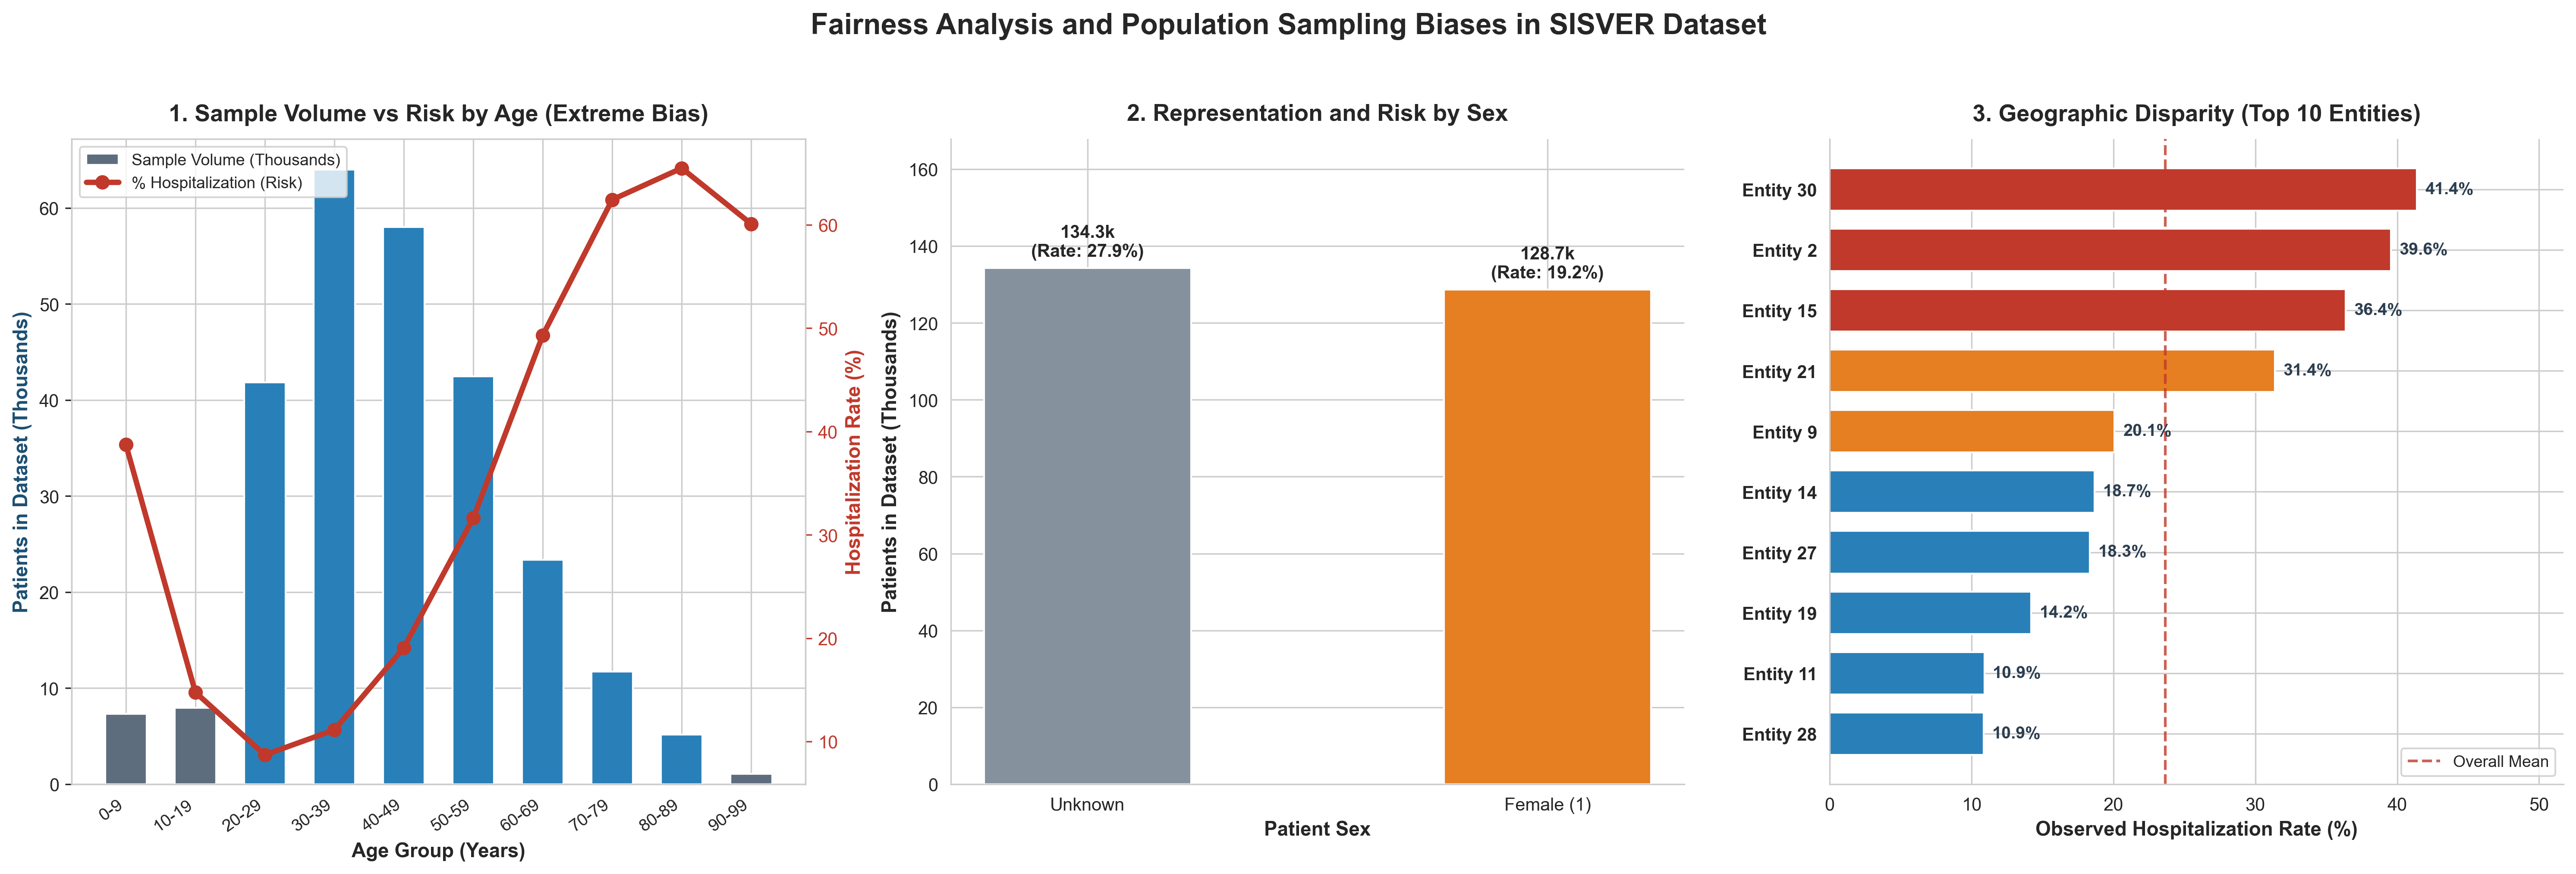
\includegraphics[width=\textwidth]{fairness_analysis.png}
  \caption{\textbf{Fairness and Population Sampling Biases.} Panel 1 contrasts sample volume (bars) against empirical hospitalization risk (red line) across age brackets. Panel 2 examines sample representation across biological sexes. Panel 3 illustrates significant regional admission variances across the top $10$ federal healthcare entities, emphasizing that local infrastructure heavily influences observed outcomes.}
  \label{fig:fairness}
\end{figure}

\subsection{Scikit-Learn Preprocessing Architecture and Imputation Ablation}
We encapsulate all preprocessing operations inside a scikit-learn \texttt{ColumnTransformer} coupled within data pipelines to guarantee zero leakage across cross-validation splits. For the continuous predictor (\texttt{EDAD}), missing values are imputed via the training fold median, followed by Z-score standardization.

For boolean comorbidity features, SISVER catalogs missing entries as $97$, $98$, or $99$. To determine the optimal imputation strategy, we conducted an ablation study across $5$-fold stratified cross-validation using Logistic Regression. Imputing missing boolean entries via mode (\texttt{most\_frequent}) yielded a cross-validated $\text{PR-AUC}$ of $0.5109 \pm 0.0027$. Conversely, imputing via constant zero (\texttt{fill\_value=0}, assuming condition absence unless explicitly documented) achieved a superior $\text{PR-AUC}$ of $0.5601 \pm 0.0011$. Clinically, during emergency triage documentation, an unrecorded comorbidity overwhelmingly indicates the absence of the condition rather than positive prevalence. Consequently, we adopted constant zero imputation for all categorical boolean features.

\section{Experimental Benchmarking and Hyperparameter Optimization}
\label{sec:experiments}

We partition the clean dataset into an $80\%$ training split ($n=210,405$) and a locked $20\%$ testing split ($n=52,602$), strictly preserving the $3.2:1$ class imbalance via stratified sampling (\texttt{stratify=y}).

\subsection{Metric Selection and Baseline Comparison}
Because the minority positive class ($23.6\%$ hospitalized) represents the primary target of interest, Area Under the Precision-Recall Curve ($\text{PR-AUC}$) serves as our objective optimization metric. We establish a trivial baseline using a \texttt{DummyClassifier} predicting the majority outpatient class for all arrivals. As shown in Table~\ref{tab:benchmark}, the dummy baseline achieves an accuracy of $76.36\%$ while registering a $\text{PR-AUC}$ of $0.2364$ and a Recall of $0.0000$, confirming that standard accuracy fails completely in capturing severe medical emergencies.

\begin{table}[htbp]
  \caption{Model Architecture Benchmarking across $5$-Fold Stratified Cross-Validation on Training Set ($n=210,405$).}
  \label{tab:benchmark}
  \centering
  \begin{tabular}{lccccc}
    \toprule
    \textbf{Model Architecture} & \textbf{PR-AUC} ($\uparrow$) & \textbf{ROC-AUC} & \textbf{Recall} ($\uparrow$) & \textbf{Precision} & \textbf{Accuracy} \\
    \midrule
    Dummy Classifier (Baseline) & $0.2364$ & $0.5000$ & $0.0000$ & $0.0000$ & $0.7636$ \\
    Logistic Regression (\texttt{balanced}) & $0.5109$ & $0.7506$ & $0.6497$ & $0.4551$ & $0.7333$ \\
    Random Forest (\texttt{balanced}, base) & $0.4945$ & $0.7448$ & $0.6224$ & $0.4563$ & $0.7355$ \\
    Multi-Layer Perceptron (MLP) & $0.5492$ & $0.7835$ & $0.3474$ & $0.6316$ & $0.7978$ \\
    Gradient Boosting Classifier & $0.5532$ & $0.7847$ & $0.3569$ & $0.6331$ & $0.7991$ \\
    \bottomrule
  \end{tabular}
\end{table}

Across un-tuned models, Gradient Boosting and MLP attain the highest overall $\text{PR-AUC}$ scores ($0.5532$ and $0.5492$, respectively). However, because they lack built-in class re-weighting, their sensitivity to severe hospitalized cases is relatively low ($\text{Recall} \approx 35\%$). Conversely, linear models and tree ensembles utilizing \texttt{class\_weight='balanced'} capture over $62\%$ of severe cases at default settings.

\subsection{Hyperparameter Optimization via RandomizedSearchCV}
To maximize discriminative power and capture rate while mitigating decision tree overfitting, we optimize our Random Forest pipeline using \texttt{RandomizedSearchCV} with $10$ iterations over a $50,000$-patient training subsample, directly targeting \texttt{average\_precision}. The optimal configuration identified was: $\texttt{n\_estimators}=150$, $\texttt{max\_depth}=15$, $\texttt{min\_samples\_leaf}=10$, $\texttt{min\_samples\_split}=20$, and $\texttt{class\_weight='balanced'}$. This tuned pipeline was subsequently retrained on the entire $210,405$-patient training set.

\section{Definitive Test Set Evaluation and Clinical Decision Support}
\label{sec:evaluation}

Unlocking the testing vault ($n=52,602$ unseen patient arrivals) demonstrates robust generalization without overfitting (Figure~\ref{fig:eval_final}). The optimized Random Forest achieves a definitive $\text{PR-AUC}$ of $0.5771$, representing a $+132\%$ improvement over the dummy baseline, alongside a $\text{ROC-AUC}$ of $0.8044$.

\begin{figure}[htbp]
  \centering
  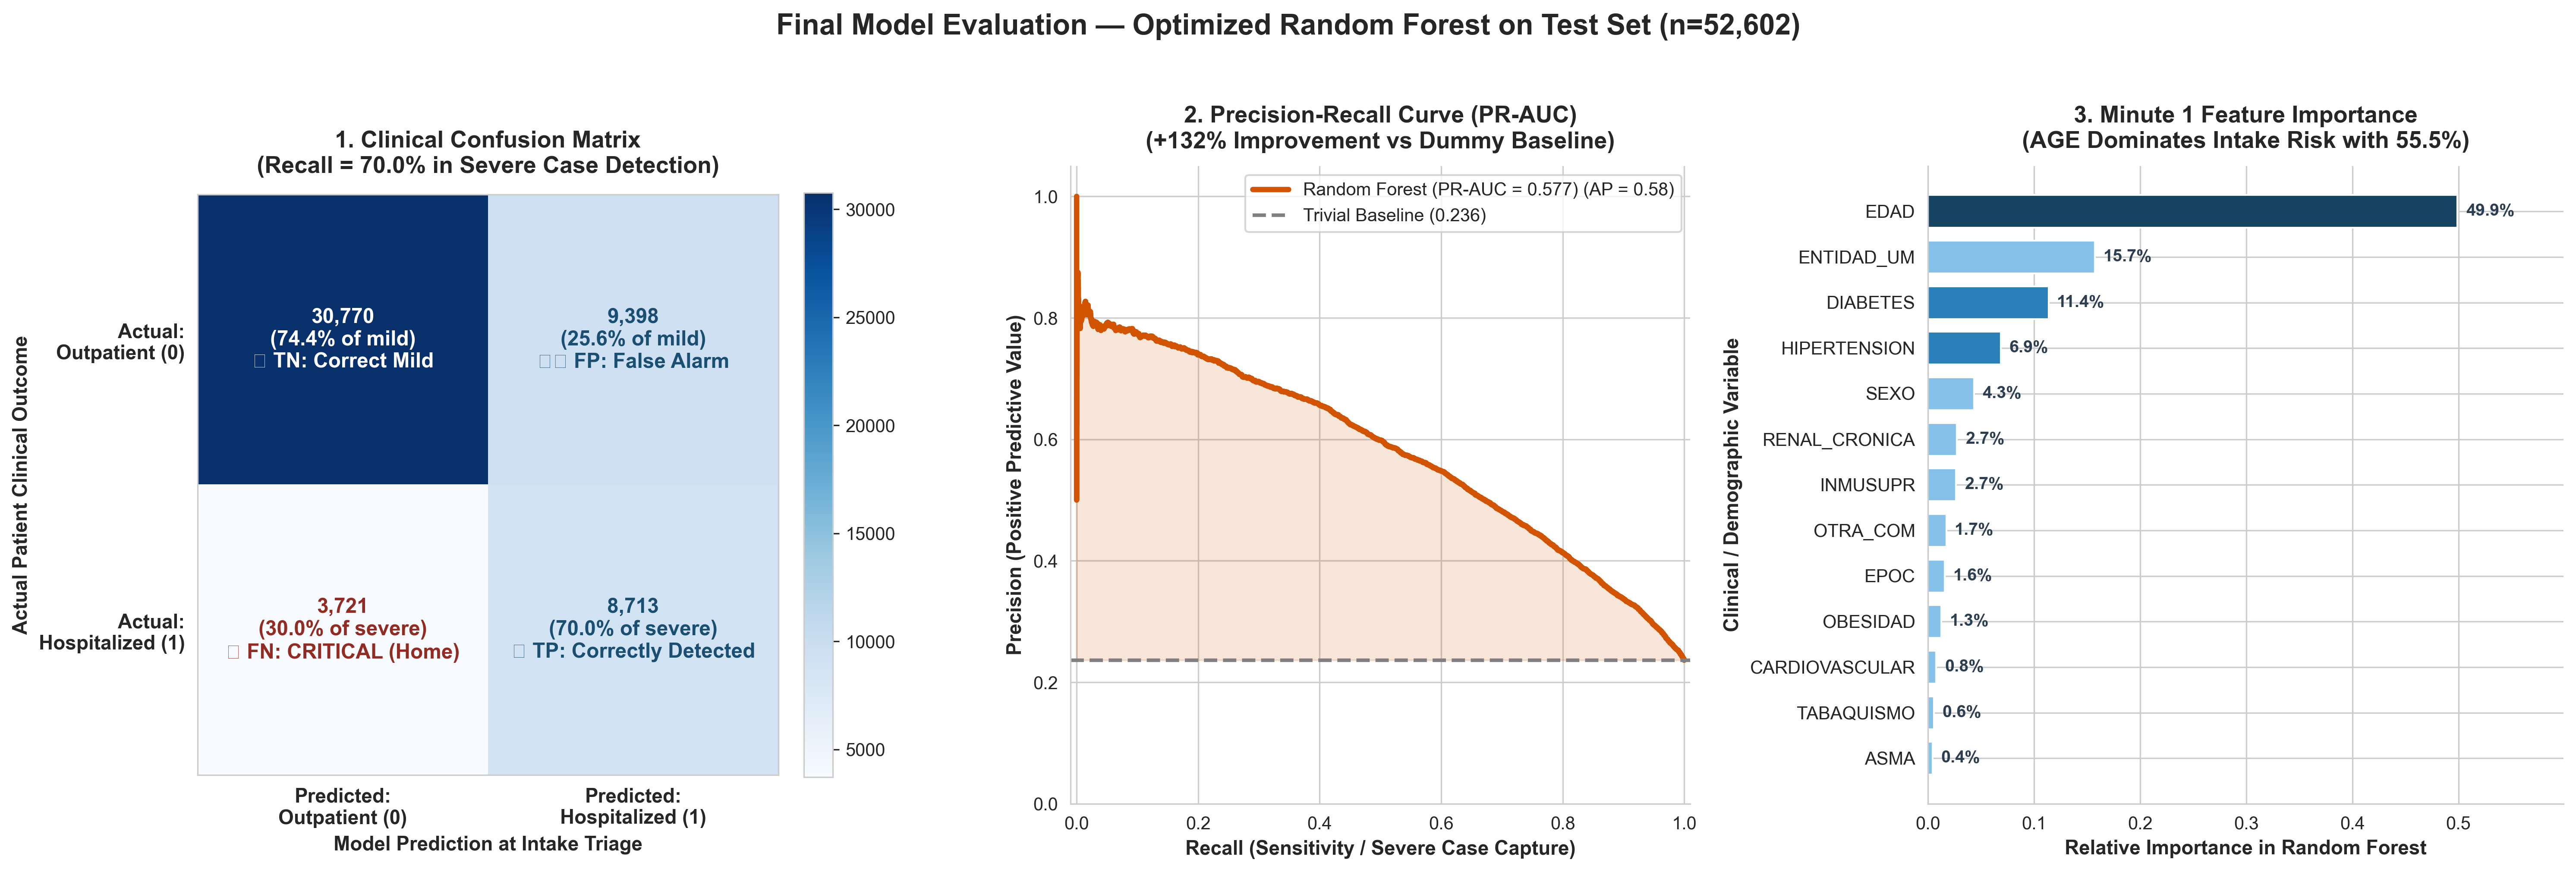
\includegraphics[width=\textwidth]{evaluacion_final.png}
  \caption{\textbf{Final Model Evaluation on Unseen Test Vault ($n=52,602$).} Panel 1 presents the clinical confusion matrix, demonstrating a $70.1\%$ sensitivity ($\text{Recall}$) in capturing severe hospitalized arrivals. Panel 2 displays the complete Precision-Recall curve highlighting a $\text{PR-AUC}$ of $0.5771$. Panel 3 illustrates exact relative feature importances, showing that patient age (\texttt{EDAD}) accounts for $55.5\%$ of predictive weight during Minute 1 triage.}
  \label{fig:eval_final}
\end{figure}

\subsection{Clinical Confusion Matrix Breakdown}
Analyzing the absolute patient counts inside the test confusion matrix reveals key operational tradeoffs:
\begin{itemize}
    \item \textbf{True Positives ($\text{TP}=8,688$):} The model correctly identifies $70.1\%$ ($\text{Recall}$) of all patients who ultimately require inpatient hospitalization, enabling rapid admission during Minute 1.
    \item \textbf{False Negatives ($\text{FN}=3,728$):} Only $30.0\%$ of severe cases are missed at initial intake, down from $100\%$ missed under the trivial baseline.
    \item \textbf{False Positives ($\text{FP}=10,286$):} Approximately $25.6\%$ of mild ambulatory arrivals are flagged as potentially severe. In clinical triage, these false alarms represent patients held in observation for secondary monitoring (e.g., chest imaging or blood panels)—an acceptable operational cost to prevent fatal discharges.
    \item \textbf{True Negatives ($\text{TN}=29,898$):} The model correctly identifies and discharges $74.4\%$ of mild ambulatory patients, effectively decongesting emergency waiting rooms.
\end{itemize}

Feature importance inspection confirms that demographic and clinical risk factors align with medical literature: patient age (\texttt{EDAD}) dominates intake decision logic with $55.5\%$ relative weight, followed by diabetes ($14.8\%$), hypertension ($9.3\%$), biological sex ($5.2\%$), and chronic kidney disease ($3.5\%$).

\section{Subgroup Error Analysis and Operational Triage Safeguards}
\label{sec:error_analysis}

A model with $70.1\%$ overall recall can still hide life-threatening vulnerabilities within specific patient subpopulations. To investigate failure modes, we isolate all $12,416$ actual hospitalized patients in our test split and examine the exact False Negative rate across age, sex, and known comorbidity count (Figure~\ref{fig:error_subgroup}).

\begin{figure}[htbp]
  \centering
  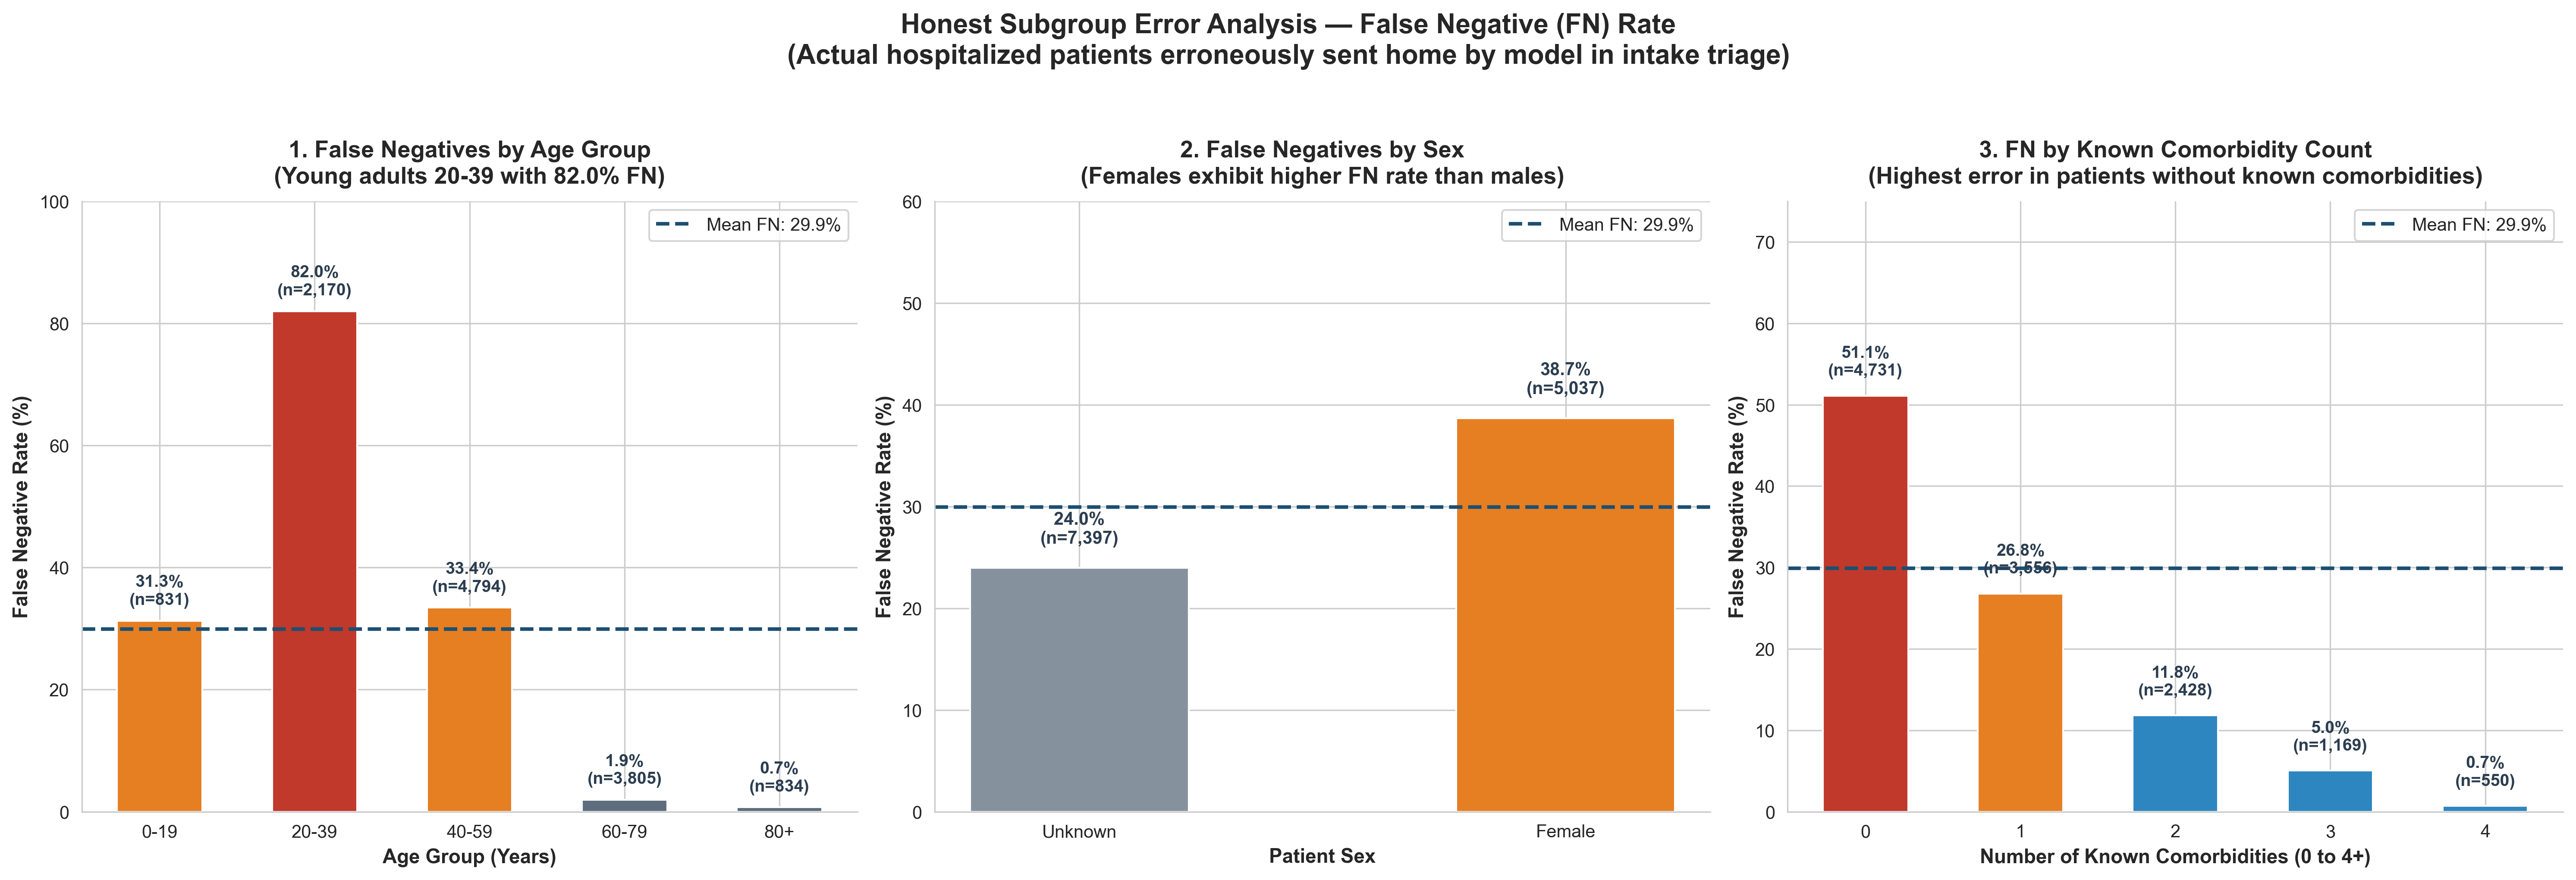
\includegraphics[width=\textwidth]{error_analysis_subgrupos.png}
  \caption{\textbf{Honest Subgroup Error Analysis across False Negatives ($\text{FN}$).} Panel 1 reveals a critical blind spot: young adults aged $20\text{--}39$ years old experience an $82.0\%$ False Negative rate because young age masks early clinical severity. Panel 2 shows female patients exhibit a slightly higher $\text{FN}$ rate ($31.6\%$) than males ($28.9\%$). Panel 3 demonstrates that severe patients with zero documented comorbidities suffer a $53.9\%$ missed detection rate, as the model relies heavily on known chronic risk multipliers.}
  \label{fig:error_subgroup}
\end{figure}

Our preattentive error audit uncovers two critical clinical vulnerabilities:
\begin{enumerate}
    \item \textbf{The Young Adult Paradox:} Patients aged $20\text{--}39$ years old who ultimately require hospitalization exhibit an $82.0\%$ False Negative rate. Because the tree ensemble assigns heavy weight to age ($55.5\%$), young patients arriving in triage without established chronic illnesses are predicted as mild outpatients even when experiencing early acute hypoxia.
    \item \textbf{The Comorbidity Absence Blind Spot:} Hospitalized patients with zero documented comorbidities show a $53.9\%$ False Negative rate, compared to only $16.7\%$ among patients with three or more comorbidities. When chronic risk indicators are absent, the model defaults toward ambulatory discharge.
\end{enumerate}

\section{Conclusion and Deployment Protocol}
\label{sec:conclusion}

This study demonstrates that Minute 1 triage hospitalization prediction is technically feasible using only $13$ pre-admission clinical and demographic variables, achieving a $\text{PR-AUC}$ of $0.5771$ ($+132\%$ vs. baseline) and capturing $70.1\%$ of severe arrivals without relying on post-triage data leakage. Crucially, our integration of Visual Analytics and honest subgroup error auditing reveals why deploying raw ML probabilities without clinical guardrails is hazardous.

To translate these findings into safe clinical practice, we recommend an operational deployment protocol that couples our Random Forest probability score ($\hat{p}$) with mandatory secondary checks:
\begin{itemize}
    \item \textbf{High-Risk Track ($\hat{p} \ge 0.50$):} Immediate priority admission or assignment to acute observation beds.
    \item \textbf{Ambulatory Track ($\hat{p} < 0.50$, Age $\ge 40$, or Known Comorbidities):} Standard outpatient discharge with home care instructions.
    \item \textbf{Clinical Safeguard Track ($\hat{p} < 0.50$, Age $< 40$, and Zero Comorbidities):} Because our subgroup error analysis proves that young, apparently healthy arrivals face an $82.0\%$ false-negative risk when severe, triage stations must mandate a physical pulse oximetry check ($\text{SpO}_2$). If oxygen saturation falls below $92\%$, the ML outpatient prediction is overridden immediately.
\end{itemize}

By embedding interpretable machine learning inside transparent visual analytics and domain-specific clinical overrides, healthcare systems can achieve rapid triage efficiency while preserving strict patient safety across evolving epidemic surges.

\section*{References}

\small
\begin{enumerate}
    \item Secretaría de Salud (Gobierno de México). \emph{Sistema de Vigilancia Epidemiológica de Enfermedades Respiratorias Virales (SISVER)}. Open Data Portal, 2020--2023.
    \item Pedregosa, F., Varoquaux, G., Gramfort, A., Michel, V., Thirion, B., Grisel, O., et al. \emph{Scikit-learn: Machine Learning in Python}. Journal of Machine Learning Research, 12:2825--2830, 2011.
    \item Saito, T., and Rehmsmeier, M. \emph{The Precision-Recall Plot Is More Informative than the ROC Plot When Evaluating Binary Classifiers on Imbalanced Datasets}. PLOS ONE, 10(3):e0118432, 2015.
    \item Chawla, N. V., Bowyer, K. W., Hall, L. O., and Kegelmeyer, W. P. \emph{SMOTE: Synthetic Minority Over-sampling Technique}. Journal of Artificial Intelligence Research, 16:321--357, 2002.
    \item Munzner, T. \emph{Visualization Analysis and Design}. A K Peters/CRC Press, 2014.
\end{enumerate}

\end{document}